%This is a experiment example of ZhengXiaoyang's experiment report template

\documentclass[UTF8]{ctexart}
 
\usepackage{amsmath}
\usepackage{cases}
\usepackage{cite}
\usepackage{xeCJK}
\usepackage{graphicx}
\usepackage[margin=1in]{geometry}
\geometry{a4paper}
\usepackage{fancyhdr}
\pagestyle{fancy}
\fancyhf{}

\graphicspath{{picture/}}


\title{拉伸法测量杨氏模量}
\graphicspath{{picture/}}


\title{拉伸法测量杨氏模量实验报告}
\author{郑晓旸}
\date{\today}
\pagenumbering{arabic}

\begin{document}
%这里是文件的开头
\fancyhead[L]{郑晓旸}
\fancyhead[C]{杨氏模量}
\fancyfoot[C]{\thepage}

\maketitle
\tableofcontents
\newpage
\section{实验原理}

在弹性范围内,物体的形变量与外力成正比。描述这种关系的参数称为杨氏模量$E$,定义为
\begin{equation}
E=\frac{F/S}{\Delta L/L}=\frac{FL}{S\Delta L}
\end{equation}
其中$F$为外力,$S$为横截面积,$L$为原长,$\Delta L$为伸长量。

本实验采用光杠杆放大法测量金属丝的伸长量。如图\ref{fig:principle}所示,待测金属丝下端与光杠杆动足相连,上端固定。施加外力$F$后,金属丝伸长$\delta L$,带动光杠杆转过角度$\delta\theta$
\begin{equation}
\delta\theta\approx\frac{\delta L}{D}
\end{equation}
其中$D$为光杠杆动足到转轴的距离。反射镜偏转$\delta\theta$后,反射光线偏转$2\delta\theta$,在标尺上的位移为
\begin{equation}
\delta x\approx 2H\delta\theta=\frac{2H}{D}\delta L
\end{equation}
其中$H$为反射镜到标尺的距离。由此可知,光杠杆的放大倍数为$K=2H/D$。

\begin{figure}[htbp]
\centering
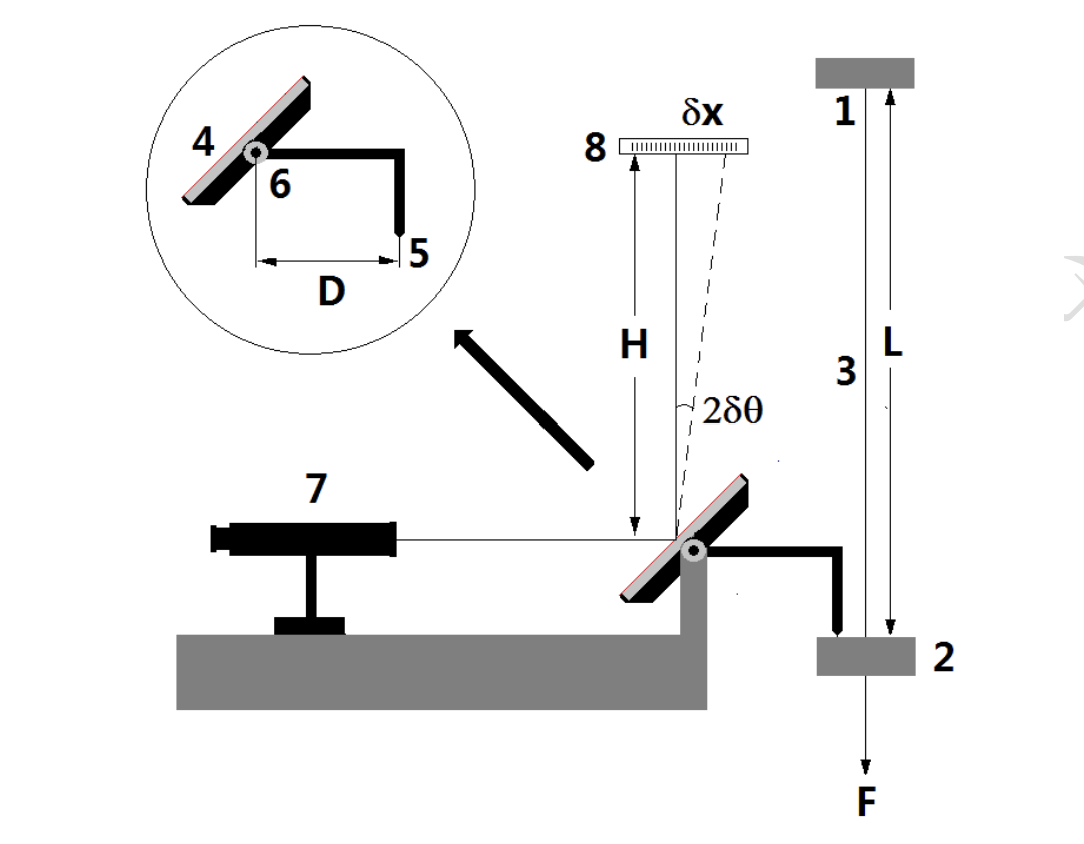
\includegraphics[width=0.6\textwidth]{principle.png}
\caption{光杠杆放大法原理图}
\label{fig:principle}
\end{figure}

将一系列外力$F_i$和对应的标尺读数$x_i$进行线性拟合
\begin{equation}
x_i=\alpha F_i+\beta
\end{equation}
然后根据斜率$\alpha$计算杨氏模量
\begin{equation}
E=\frac{8LH}{\pi d^2D\alpha}
\end{equation}
其中$d$为金属丝直径。

\section{实验过程}
\begin{enumerate}
    \item 调节测试架,连接信号线,打开数字拉力计,预热10min。
    \item 调节望远镜,使视野清晰,十字分划线与标尺刻度平行。
    \item 测量金属丝原长$L$、反射镜到标尺距离$H$、光杠杆常数$D$和金属丝直径$d$。
    \begin{enumerate}
        \item 用千分尺测量金属丝直径$d$。在不同位置测量10次,数据如下:
        \\
        \begin{table}[htbp]
        \centering
        \begin{tabular}{|l|}
        \hline
        d(mm)\\
        \hline
        0.70\\
        \hline
        0.70\\
        \hline
        0.70\\
        \hline
        0.70\\
        \hline
        0.70\\
        \hline
        0.71\\
        \hline
        0.70\\
        \hline
        0.71\\
        \hline
        0.70\\
        \hline
        0.70\\
        \hline
        \end{tabular}
        \end{table}
        \item 使用卷尺和游标卡尺测量测量金属丝原长 L、反射镜到标尺距离 H,以及光杠杆长度D。数据如下:   
        \\
        \begin{table}[htbp]
        \centering
    \begin{tabular}{|l|l|l|}
        \hline
    L(mm)&H(mm)&D(mm)\\
    \hline
    764.0&703.0&34.56\\
    \hline
    \end{tabular}
    \end{table}

    \end{enumerate}
    \item 缓慢旋转施力螺母,每隔1kg记录一次标尺读数,测量加力和卸力两个过程。
    \begin{enumerate}
        \item 施力过程由0.51kg开始,每隔1kg记录一次标尺读数,直至10.51kg。
        \item 然后加至11.51kg,松弛一部分。
        \item 从10.21kg开始记录,每隔1kg记录一次标尺读数,直至0.34kg。
        \item 记录数据如下图\ref{fig:origin}:
        \begin{figure}[htbp]
            \centering
            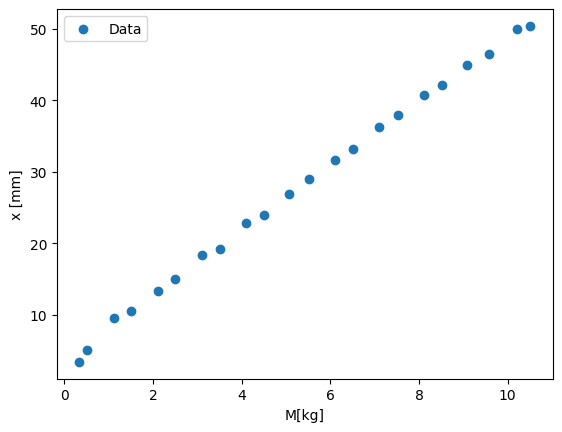
\includegraphics[width=0.4\textwidth]{origin.png}
            \caption{原始测量数据}
            \label{fig:origin}
            \end{figure}
    \end{enumerate}
    \newpage
    \item 数据处理,根据公式(3)计算$\delta L=\frac{D\delta x}{2H}$和拉力$F=Mg$。
    \item 数据处理,线性拟合$F_i-x_i$,结果如下图\ref{fig:fitting},计算杨氏模量$E$及其不确定度$u(E)$。
    \begin{figure}[htbp]
        \centering
        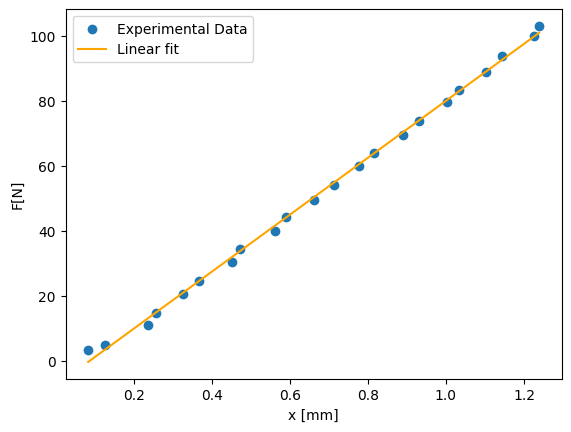
\includegraphics[width=0.4\textwidth]{fitting.png}
        \caption{拟合结果}
        \label{fig:fitting}
    \end{figure}
\end{enumerate}

\section{实验结果和数据分析}
\subsection{实验结果}
根据公式(1),由钢丝伸长量$\delta L$和所受外力$F$的关系,得到计算杨氏模量$E$的公式:
\begin{equation}
    E=\frac{F/S}{\Delta L/L}=\frac{4FL}{\pi d^2 \Delta L}
\end{equation}
由拟合得到的:$F/\delta L= 87.5849 N/mm$
计算得到杨氏模量$E=173 \pm 2 \ GPa$。
\subsection{误差分析}
\begin{enumerate}
    \item 金属丝直径$d$的不确定度为$u(d)=\sqrt{\frac{\sigma(d_i-\bar{d})^2}{n(n-1)}+\frac{0.001}{\sqrt{3}}}=0.0038mm$。
    \item 金属丝原长$L$、反射镜到标尺距离$H$、光杠杆长度$D$的不确定度为$u(L)=u(H)=u(D)=0.6mm$。
    \item 金属丝拉力与伸长量比值$F/\delta L$的不确定度为$u(F/\delta L)=\sqrt{\frac{\frac{1}{r^2}-1}{n-2}}=0.80N/mm$。
    \item 由公式(3)和(4)计算得到杨氏模量$E$的不确定度为
    \begin{equation}
    \frac{u(E)}{E}=\sqrt{(\frac{u(F/ \delta L)}{F/ \delta L})+(\frac{u(L)}{L})+(\frac{2u(d)}{d})^2}=1.42\%
    \end{equation}
\end{enumerate}
\subsection{讨论}
\begin{enumerate}
    \item 与理论值比较
    钢的杨氏模量约为210GPa,本实验测得的杨氏模量为173GPa,与理论值相差较大。可能的原因有:实验用金属丝不是结构钢丝,而是精钢丝,或者蒙乃尔合金丝。
    \item 实验中的不确定度
    本实验中的主要不确定度来源是金属丝直径$d$的测量误差,其次是金属丝拉力与伸长量比值$F/\delta L$的测量误差。通过减小这两项误差,可以提高实验结果的精度。
    \item 实验中的系统误差
    本实验中的系统误差主要来源是金属丝的弯曲和滞弹性。通过预拉金属丝,可以消除弯曲的影响;通过测量加卸载两个过程的拉伸,可以消除滞弹性的影响。
\end{enumerate}
\section{附录}
\subsection{原始数据}
见附页
\end{document}
